\section{Diagrama de clases del análisis} % (fold)
\label{sec:diagrama_de_clases_analisis}

\subsection{Actividades generales} % (fold)
\label{sub:actividades_generales}
	
	En primer lugar podemos ver el diagrama referente a los nuevos registros tanto de pacientes como de médicos (Figura \ref{fig:col_clase7}).
	\begin{figure}[H]
	  \centering
	    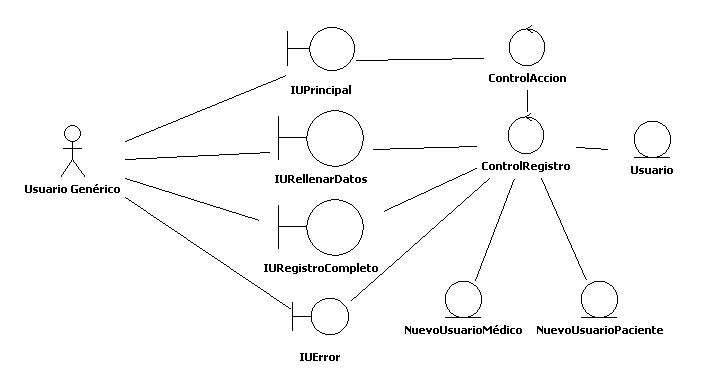
\includegraphics[width=15cm, height= 7cm]{img/jpg/clases/7_Registrarse.jpg}
	  \caption{Registrarse}
	  \label{fig:col_clase7}
	\end{figure}

	Una vez realizado el registro, se deben rellenar una serie de datos (Figura \ref{fig:col_clase8})
	\begin{figure}[H]
	  \centering
	    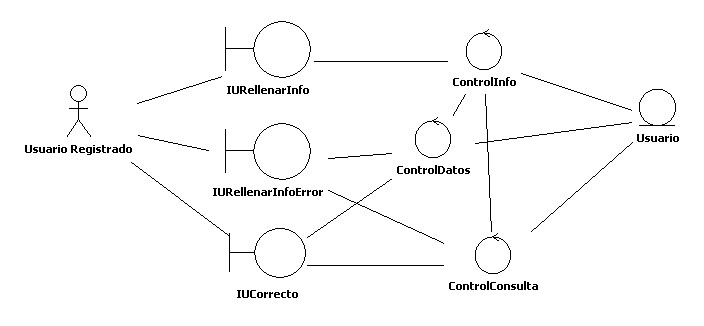
\includegraphics[width=15cm, height=7cm]{img/jpg/clases/7_RellenarInfo.jpg}
	  \caption{Rellenar información}
	  \label{fig:col_clase8}
	\end{figure}
	
	A continuación un diagrama muy general (Figura \ref{fig:col_clase9}), en el que se muestran el resto de actividades generales que pueden realizar los usuarios genéricos. Éstas son buscar médico, términos legales, condiciones de uso, contactar con el administrador, preguntas frecuentes y cambiar idioma.
	\begin{figure}[H]
	  \centering
	    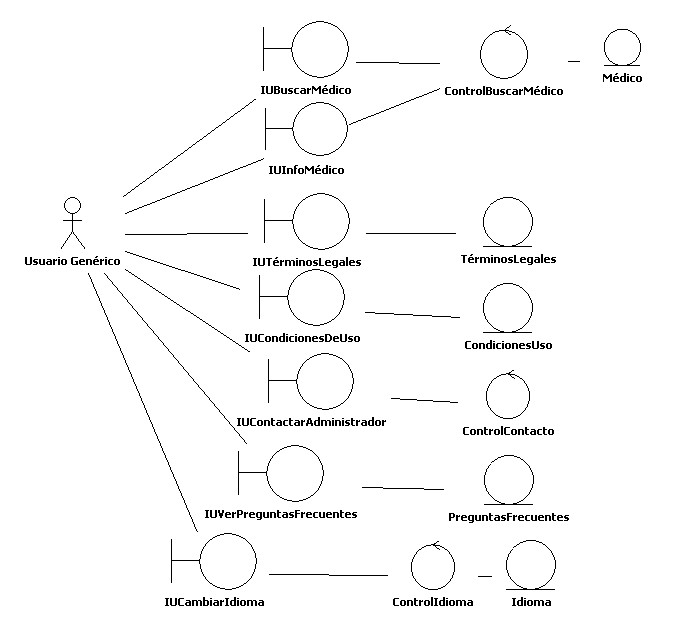
\includegraphics[width=16cm]{img/jpg/clases/8_Varios.jpg}
	  \caption{Otras actividades}
	  \label{fig:col_clase9}
	\end{figure}
	
	\newpage
	Por último, el diagrama relacionado con el acceso y autentificación (Figura \ref{fig:col_clase10}) para iniciar una nueva sesión. Tras el acceso, se va al dashboard del médico o del paciente
	\begin{figure}[H]
	  \centering
	    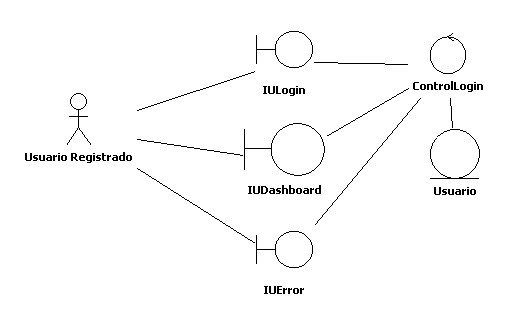
\includegraphics[width=12cm]{img/jpg/clases/9_AccesoYAutentificacion.jpg}
	  \caption{Acceso y autentificación}
	  \label{fig:col_clase10}
	\end{figure}

% subsection actividades_generales (end)

\newpage
\subsubsection{Médicos} % (fold)
\label{ssub:medicos}

	En primer lugar podemos ver todo lo relacionado con la configuración del médico (Figura \ref{fig:col_clase1}), que a su vez se verá con más detalle en los siguientes diagramas. Las posibles cosas que se pueden configurar son la información, la cuenta, el horario, las notificaciones y los motivos.
	\begin{figure}[H]
	  \centering
	    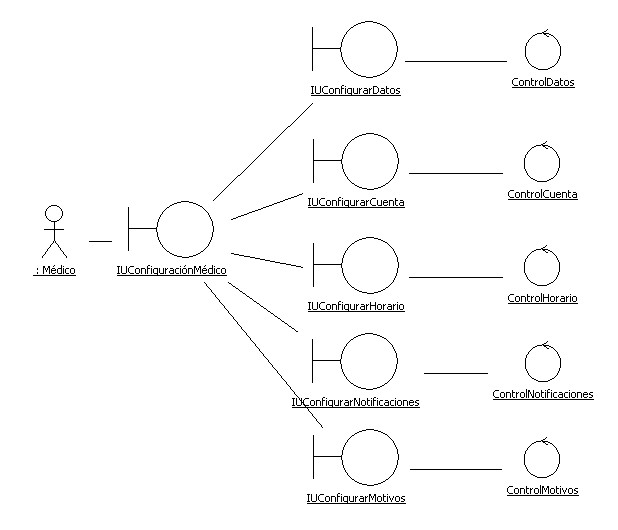
\includegraphics[width=16cm]{img/jpg/clases/1_MedicoConfiguracion.jpg}
	  \caption{Configuración del médico}
	  \label{fig:col_clase1}
	\end{figure}
	
	\newpage
	A la hora de configurar los datos (Figura \ref{fig:col_clase2}), en principio, serán los datos personales, los de localización y los de contacto.
	\begin{figure}[H]
	  \centering
	    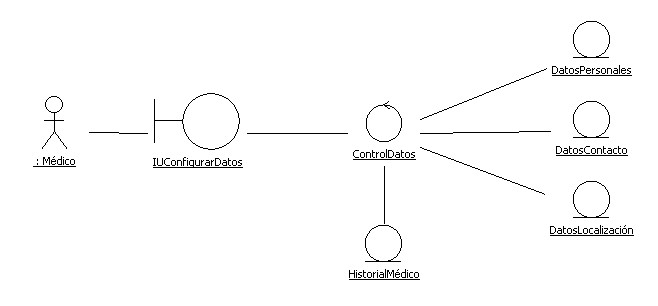
\includegraphics[width=12cm, height=5cm]{img/jpg/clases/2_MedicosConfiguracionDatos.jpg}
	  \caption{Configuración de los datos del médico}
	  \label{fig:col_clase2}
	\end{figure}

	En la configuración de la cuenta (Figura \ref{fig:col_clase3}), observamos que principalmente se puede cambiar el email, la contraseña y el idioma. Además, podrá darse de baja del servicio. Si se modifica la configuración, se guardará un registro en el \textit{historial del médico}.
	\begin{figure}[H]
	  \centering
	    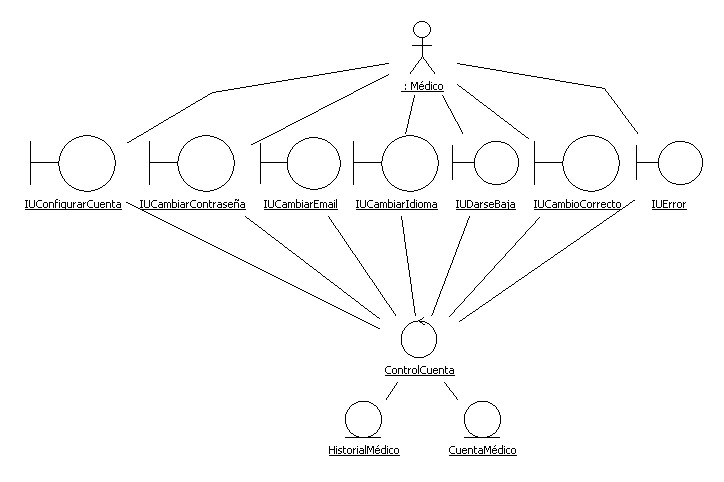
\includegraphics[width=16cm, height=10cm]{img/jpg/clases/3_MedicoConfiguracionCuenta.jpg}
	  \caption{Configuración de la cuenta del médico}
	  \label{fig:col_clase3}
	\end{figure}
	
	Un médico también podrá configurar su horario (Figura \ref{fig:col_clase4}).
	\begin{figure}[H]
	  \centering
	    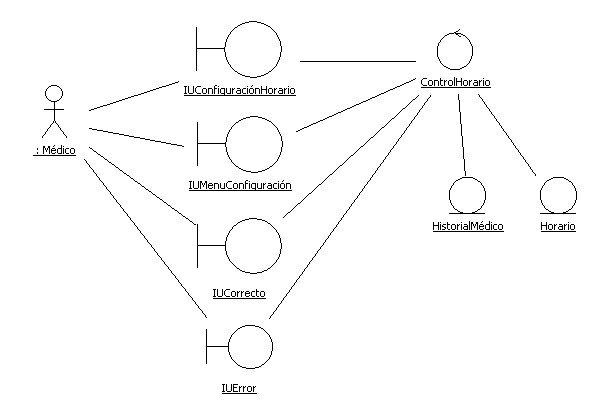
\includegraphics[width=12cm, height=6cm]{img/jpg/clases/4_MedicoConfiguracionHorario.jpg}
	  \caption{Configuración del horario del médico}
	  \label{fig:col_clase4}
	\end{figure}

	Por otro lado, un médico tiene que poder ser capaz de ver sus calendarios (Figura \ref{fig:col_clase5}), en distintos tipos de vista. En ellos aparecerán las citas que tienen concertadas, y debe ser capaz de anular una concreta o de ver la información de la ficha médica de sus pacientes. Además, al anular una cita se le enviará un mensaje al paciente.
	\begin{figure}[H]
	  \centering
	    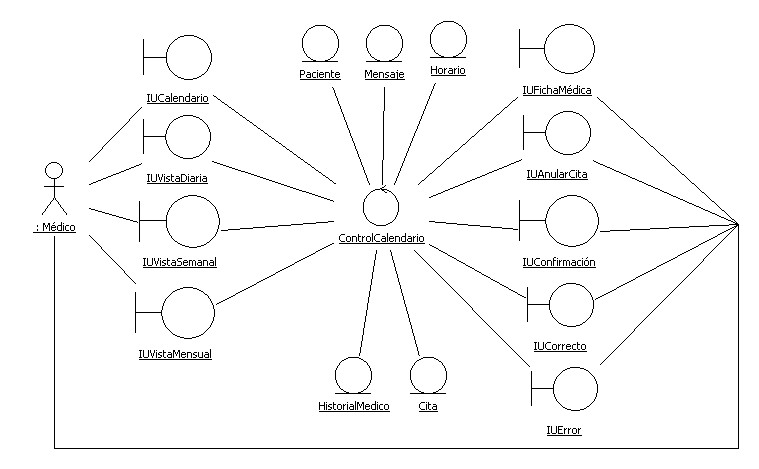
\includegraphics[width=16cm, height=9cm]{img/jpg/clases/5_CalendarioMedico.jpg}
	  \caption{Calendario del médico}
	  \label{fig:col_clase5}
	\end{figure}
	
	
	El último de los principales diagramas de clases relacionados con los médicos es el de sus pacientes (Figura \ref{fig:col_clase6}). Podrá buscarlos de distintas maneras y ver su información.
	\begin{figure}[H]
	  \centering
	    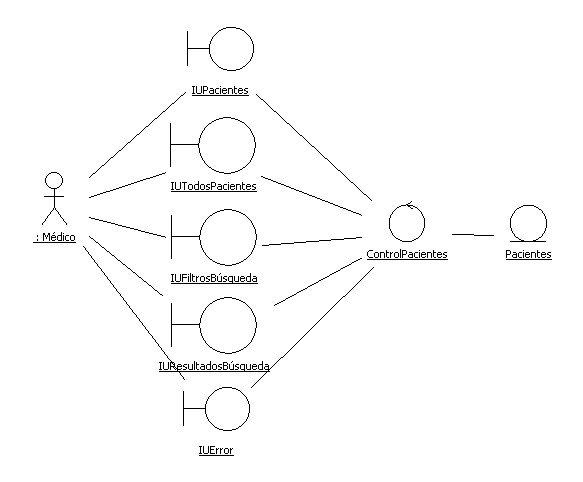
\includegraphics[width=16cm]{img/jpg/clases/6_MedicosPacientes.jpg}
	  \caption{Pacientes del médico}
	  \label{fig:col_clase6}
	\end{figure}

% subsubsection médicos (end)

\newpage
\subsection{Pacientes} % (fold)
\label{sub:pacientes}

Respecto a los pacientes, los diagramas de clases relacionados con la configuración de los datos y de la información son prácticamente iguales que los diagramas de los médicos.

Por otro lado, un paciente tiene que poder ser capaz de ver sus calendarios (Figura \ref{fig:col_clase11}), en distintos tipos de vista. En ellos aparecerán las citas que tienen concertadas, y debe ser capaz de anular una concreta o de ver la información de sus médicos. Además, al anular una cita se le enviará un mensaje al médico.
\begin{figure}[H]
  \centering
    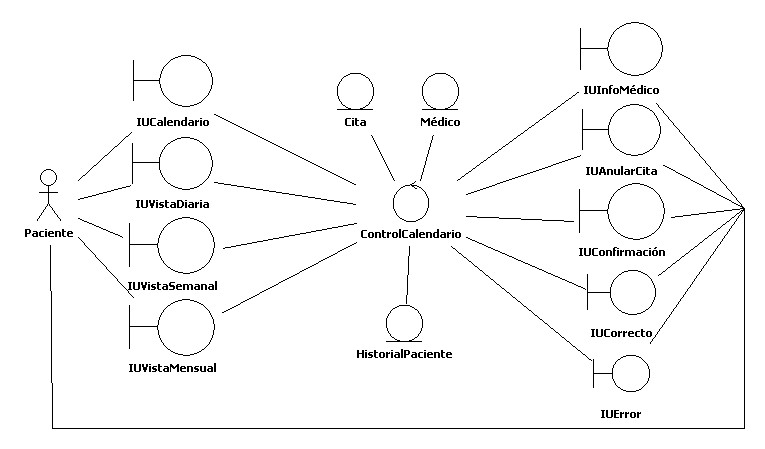
\includegraphics[width=16cm]{img/jpg/clases/10_PacientesCalendario.jpg}
  \caption{Calendario del paciente}
  \label{fig:col_clase11}
\end{figure}

\newpage
El último de los principales diagramas de clases relacionados con los pacientes es el de sus médicos (Figura \ref{fig:col_clase12}). Podrá buscarlos de distintas maneras y ver su información y sus horarios.
\begin{figure}[H]
  \centering
    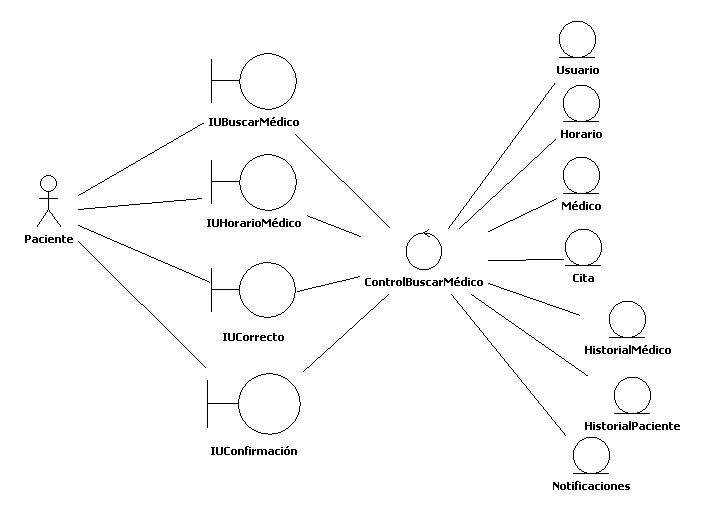
\includegraphics[width=16cm]{img/jpg/clases/11_PacientesMedicos.jpg}
  \caption{Buscar los médicos de un paciente}
  \label{fig:col_clase12}
\end{figure}
% subsection pacientes (end)

\newpage
\subsection{Ficha médica} % (fold)
\label{sub:ficha_medica}

	Una ficha médica abarca muchos tipos de datos y de pruebas. Entre otros, los antecedentes (de diversos tipos), diagnósticos, tratamientos, pruebas etcétera. En el primer diagrama (Figura \ref{fig:col_clase13}) vemos en detalle lo relacionado con los antecedentes.
	\begin{figure}[H]
	  \centering
	    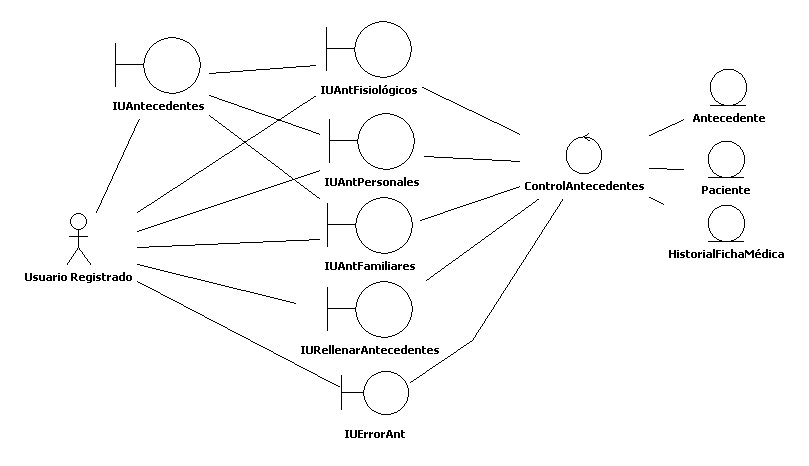
\includegraphics[width=16cm]{img/jpg/clases/12_Antecedentes.jpg}
	  \caption{Antecedentes}
	  \label{fig:col_clase13}
	\end{figure}

	\newpage
	En este diagrama (Figura \ref{fig:col_clase14}) encontramos lo relacionado con los informes, los tratamientos, los diagnósticos y las distintas posibles exploraciones clínicas.
	\begin{figure}[H]
	  \centering
	    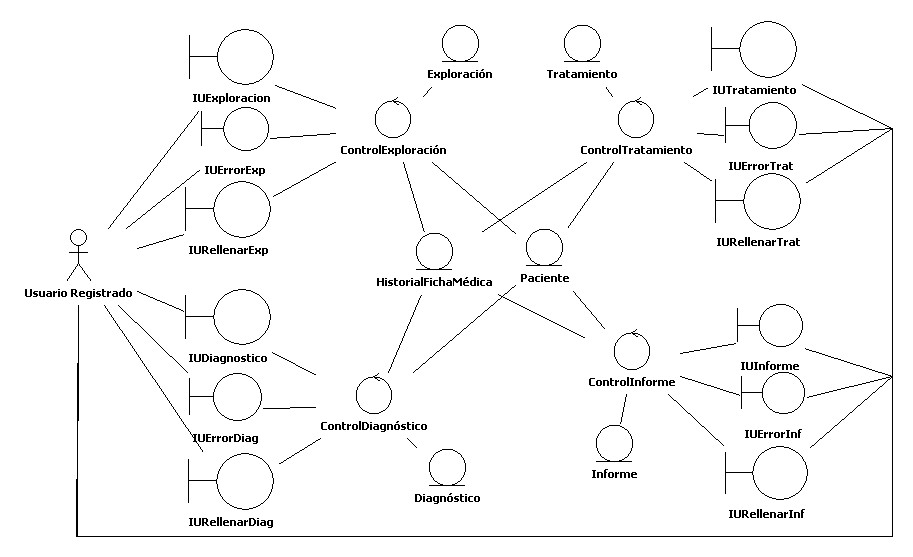
\includegraphics[width=16cm]{img/jpg/clases/13_Resto.jpg}
	  \caption{Resto de casos.}
	  \label{fig:col_clase14}
	\end{figure}
% subsection ficha_médica (end)
	
\newpage
\subsection{Administrador} % (fold)
\label{sub:administrador}
	Por último tenemos el diagrama de clases relacionado con el administrador del sistema. Éste podrá habilitar médicos, suspenderlos, verificar su licenciatura, responder a las preguntas de los usuarios, agregar nuevos administradores, modificar el contenido de los términos legares y de las condiciones de uso.
	\begin{figure}[H]
	  \centering
	    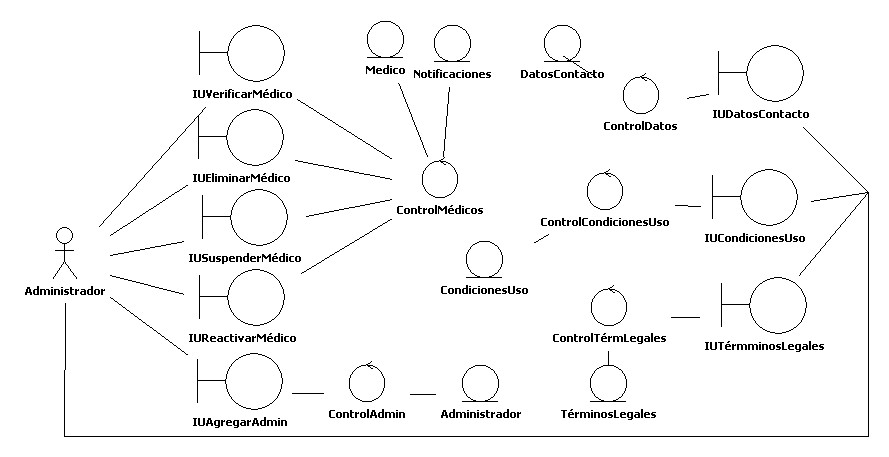
\includegraphics[width=16cm]{img/jpg/clases/14_Administrador.jpg}
	  \caption{Registrarse como paciente}
	  \label{fig:col_clase15}
	\end{figure}
	
% subsection administrador (end)

% section diagrama_de_clases (end)

